\documentclass[10pt,a4paper]{article}
\usepackage{fontspec}
\setmainfont{Times New Roman}\setsansfont{Helvetica}\setmonofont{Courier New}
\usepackage[margin=2.5cm]{geometry}
\usepackage{graphicx,booktabs,caption,setspace,tabularx,longtable,float,enumitem,amsmath}
\usepackage[hidelinks,breaklinks=true]{hyperref}
\emergencystretch=3em
\usepackage{titlesec}
\titleformat{\section}{\large\bfseries}{}{0em}{}
\titleformat{\subsection}{\normalsize\bfseries}{}{0em}{}
\renewcommand{\thefigure}{S\arabic{figure}}
\renewcommand{\thetable}{S\arabic{table}}

\title{\Large\textbf{Supplementary Appendix}\\[6pt]\large Domestic Government Health Expenditure, Out-of-Pocket Spending, and\\ Healthy Life Expectancy in 190 Countries, 2000--2022}
\author{Qingqing Mo\textsuperscript{1,2}, Pingbo Chen\textsuperscript{1,2}, Cheng Xu\textsuperscript{1,2}, Ya Wang\textsuperscript{1,2}, Ting Hu\textsuperscript{1,2},\\ Qian Sun\textsuperscript{1,2}, Tao Zhu\textsuperscript{1,2*}}
\date{\footnotesize\begin{itemize}[leftmargin=*,nosep]
\item 1. Department of Obstetrics and Gynecology, National Clinical Research Center for Obstetrics and Gynecology, Tongji Hospital, Tongji Medical College, Huazhong University of Science and Technology, Wuhan, China
\item 2. Key Laboratory of Cancer Invasion and Metastasis, Ministry of Education, Tongji Hospital, Tongji Medical College, Huazhong University of Science and Technology, Wuhan, China
\item * Correspondence: zhutao@tjh.tjmu.edu.cn
\end{itemize}}

\begin{document}
\maketitle

\noindent\textit{These materials support the main analyses and are not required for understanding the primary findings.}
\textbf{Tables.} S1 (sample characteristics), S2 (country coverage; incl. S2b country list), S3 (descriptive statistics), S4 (robustness specifications; incl. S4b sequential coefficients, S4c pre-COVID and era splits), S5 (synthetic control diagnostics), S6 (long-difference analysis), S7 (GHE spike events), S8 (austerity episodes; incl. S8b stacked event study), S9 (low-income sensitivity and bootstrap), S10 (MDE and exclusion testing), S11 (three-pipeline convergence), S12 (temporal heterogeneity), S13 (standardised-coefficient model), S14 (included studies), S15 (alternative outcomes), S16 (reform case studies).\par
\textbf{Figures.} S1 (search flow), S2 (event study excluding COVID-era spikes), S3 (coefficient forest plot), S4 (temporal aggregation), S5 (regional heterogeneity), S6 (SCM gap plots), S7 (placebo event study), S8 (income-stratified standardised coefficients), S9--S12 (low-income analyses, enlarged versions of the panels composing Figure 3), S13 (pathway decomposition), S14 (event studies around GHE spikes and austerity).

\section{Supplementary Methods}

\subsection{Structured Literature Search}
The structured search was conducted in PubMed (MEDLINE) through the NCBI E-utilities interface on August 14, 2026, using the query: (``government health expenditure'' OR ``public health spending'' OR ``health financing'') AND (``life expectancy'' OR ``mortality'' OR ``population health'') AND (``governance'' OR ``institutional quality'' OR ``causal identification'' OR ``fixed effects'' OR ``panel''), restricted to publications from January 1, 2000 to August 14, 2026. The search returned 155 records; no duplicates were identified within the single database. All 155 records were screened on title and abstract. Inclusion criteria were: (i) country-level panel or cross-sectional design; (ii) government or public health expenditure as a primary exposure; (iii) life expectancy, HALE, or mortality as an outcome. Exclusion criteria were: (i) no government health expenditure exposure ($n = 16$); (ii) sub-national design only ($n = 31$); (iii) no health outcome ($n = 18$); (iv) review or commentary without original analysis ($n = 61$). A total of 126 records were excluded and 29 studies were included in the evidence synthesis (Figure S1). The complete screening ledger, with the decision and reason for every record, is provided in the replication package (screening\_records.csv).

\subsection{Data Sources and Variable Construction}
HALE at birth was extracted from the GBD 2023 Results Tool
(\url{https://vizhub.healthdata.org/gbd-results/}, accessed July 19,
2026). Government health expenditure (SH.XPD.GHED.GD.ZS) and external health expenditure (SH.XPD.EHEX.CH.ZS, downloaded August 10, 2026) were obtained from the World Bank WDI API. Additional WDI variables: infant mortality (SP.DYN.IMRT.IN), GDP per capita PPP (NY.GDP.PCAP.PP.KD), urban population (SP.URB.TOTL.IN.ZS), fertility rate (SP.DYN.TFRT.IN), and out-of-pocket expenditure (SH.XPD.OOPC.CH.ZS). Tax revenue (GC.TAX.TOTL.GD.ZS) from the IMF GFS and WDI. The governance composite is the equal-weighted mean of six WGI 2025 dimensions (Cronbach's $\alpha$ = 0{\textperiodcentered{}}97; \url{https://www.govindicators.org}). The World Bank's most recent income classification available at data extraction (July 2026 data vintage) was applied as a time-invariant attribute to avoid group-switching bias. The full country-to-group mapping is provided in the replication package.

\subsection{Analytical Pipelines}
Three analytical pipelines were implemented: (i) multiple imputation (20 imputed datasets); (ii) complete-case analysis; and (iii) the primary pipeline, which included event studies, synthetic control, mediation, temporal aggregation, and the comparative standardised-coefficient model. All analyses were performed in R 4.5.0 using the following packages: \texttt{fixest} 0.13.1 (two-way fixed effects estimation), \texttt{data.table} 1.16.4 (data management), \texttt{tidysynth} 0.2.0 (synthetic control), \texttt{mice} 3.17.3 (multiple imputation), \texttt{ggplot2} 3.5.1 (graphics), and \texttt{fwildclusterboot} 0.13.0 (wild cluster bootstrap). Random seed 49 was used for all stochastic procedures.

\subsection{Minimal Detectable Effect and One-Sided Exclusion Testing}
MDE at 80\% power and $\alpha = 0{\textperiodcentered{}}05$ (two-sided), using the clustered standard error from the primary TWFE specification ($N = 4{,}304$, $G = 189$), was calculated as
\begin{equation}
\text{MDE} = (z_{1-\alpha/2} + z_{1-\beta}) \times \text{SE}_{\text{TWFE}} = 2{\textperiodcentered{}}80 \times 0{\textperiodcentered{}}068 = 0{\textperiodcentered{}}19
\end{equation}
HALE-years per percentage point of GDP. One-sided exclusion testing followed the two one-sided tests framework (ref S2), testing $H_0: \beta \geq \delta$ against $H_1: \beta < \delta$ for exclusion bounds $\delta \in \{0{\textperiodcentered{}}1, 0{\textperiodcentered{}}2\}$. The exclusion bound of $+0{\textperiodcentered{}}1$ HALE-years per percentage point of GDP was chosen as a conservative threshold representing approximately 7\% of the cross-sectional gradient ($+1{\textperiodcentered{}}47$), well below what would be considered a policy-meaningful effect. The null hypothesis $\beta \geq +0{\textperiodcentered{}}2$ was rejected at $p < 0{\textperiodcentered{}}001$ and $\beta \geq +0{\textperiodcentered{}}1$ at $p = 0{\textperiodcentered{}}0006$.

\subsection{Wild Cluster Bootstrap}
We implemented a cluster wild bootstrap (ref S1) for the low-income TWFE specification to address the small number of clusters ($G = 23$ after listwise deletion). The bootstrap procedure applied cluster-level Rademacher weights ($\pm 1$ with equal probability) to the model scores under the null hypothesis, re-estimating the full TWFE model on each of $B = 9{,}999$ replications (random seed 49; studentised bootstrap-t statistic). The two-sided bootstrap-t $p$-value (0{\textperiodcentered{}}065) was computed from the studentised bootstrap distribution; bootstrap-based confidence intervals were unstable with 23 clusters and are therefore not reported. This approach provides asymptotic refinement over standard cluster-robust inference when the number of clusters is small.

\subsection{Leave-One-Out Jackknife}
For both the full sample ($G = 189$ countries in the complete-case set) and the low-income subsample ($G = 23$ countries), we iteratively excluded each country and re-estimated the primary TWFE specification. The range of resulting GHE coefficients quantifies the influence of any single country on the overall estimate. For the low-income analysis, this is particularly important given the small number of clusters: a single influential country could drive the positive signal. The leave-one-out procedure is also a non-parametric sensitivity check that does not rely on asymptotic approximations.

\subsection{Additional Methodological Details}
\subsubsection{Missing Data}
Missingness is reported on the merged panel of 4,314 country-years (after excluding World Bank aggregate entities and records with incomplete exposure or outcome data): HALE, GHE, and GDP per capita were complete (0\% missing); urbanisation 0{\textperiodcentered{}}2\%, fertility 0{\textperiodcentered{}}2\%, governance 4{\textperiodcentered{}}8\%, out-of-pocket expenditure 0{\textperiodcentered{}}2\%, and tax revenue 36{\textperiodcentered{}}0\%. Because the primary covariates are nearly complete, listwise deletion across them retains the primary analysis sample of 4,304 country-years (99{\textperiodcentered{}}8\% of the raw panel), used by both the primary TWFE and the pathway decomposition; adding governance reduces the sample to 4,098 (a further 4{\textperiodcentered{}}8\%). IV-2SLS restricted to non-missing tax revenue ($N = 2{,}753$). Pipeline (i) (multiple imputation) used MICE ($m = 20$, PMM; ref S3) as sensitivity. The pattern of missingness was not completely at random: governance data were more frequently missing for smaller and lower-income countries. However, the consistency of results across complete-case and MICE-based analyses suggests that missing-data bias is unlikely to materially affect the conclusions.

\subsubsection{Instrumental Variable Analysis (pre-specified, unsuccessful)}
Tax revenue failed as instrument within-country (first-stage F $< 0{\textperiodcentered{}}2$ in TWFE). One pipeline's long-difference specification produced F $= 16{\textperiodcentered{}}3$ but wide second-stage CIs ($-1{\textperiodcentered{}}27$ to $+0{\textperiodcentered{}}61$). The failure of the within-country IV strategy reflects the fact that year-to-year variation in tax revenue is dominated by macroeconomic cycles rather than structural fiscal capacity changes, making it a weak predictor of within-country GHE variation.

\subsubsection{Event Study Specification}
The event-study equation follows the main text (equation 2), with covariates $\mathbf{X}_{it}$ comprising log GDP per capita, urbanisation, and fertility. $t_i^*$ = first GHE spike year ($>2$ percentage points [pp] of GDP within any 3-year window), $k = -5$ is the reference period. Pre-trend coefficients ($k = -4$ to $-1$) were not significant ($p > 0{\textperiodcentered{}}3$ for all), supporting the parallel trends assumption. Standard errors clustered at country level. Because treatment timing is staggered, we additionally estimated a stacked event study (16 pre-2020 cohorts, cohort-by-period fixed effects, clean controls): post-spike point estimates remained negative (post-average $-0{\textperiodcentered{}}31$; $t+5$: $-0{\textperiodcentered{}}39$, $p = 0{\textperiodcentered{}}45$) but were not conventionally significant, and one pre-trend coefficient ($k = -4$) was significant in that stacked specification, reinforcing the descriptive interpretation of the event-study evidence (Table S8b).

\subsubsection{Exploratory Pathway Decomposition}
Product-of-coefficients method under TWFE (ref S15). OOP is modelled in natural-log form ($\ln(\text{OOP} + 0{\textperiodcentered{}}01)$), so coefficient $a$ is a semi-elasticity: each 1-percentage-point increase in GHE (share of GDP) is associated with an approximate 11\% relative reduction in the OOP share of current health expenditure. All estimates are complete-case; the pathway equations follow the main text (equations 3 and 4).
Indirect effect (GHE $\rightarrow$ OOP $\rightarrow$ HALE): $a \times b = +0{\textperiodcentered{}}100$. Direct effect: $c' = -0{\textperiodcentered{}}222$. Total effect: $c = -0{\textperiodcentered{}}122$. The positive indirect effect through OOP reduction partially offsets the negative direct effect, compatible with the interpretation that GHE is associated with improved financial protection even where it is not associated with measurable health outcomes. Catastrophic and impoverishing health expenditure indicators (SDG 3{\textperiodcentered{}}8{\textperiodcentered{}}2 and its companion impoverishment metric) are survey-based with irregular country coverage and could not be analysed as annual panels; the OOP share therefore provides the financing-mix proxy for financial protection.

\subsubsection{Data and Code Availability}
All data publicly available. GBD 2023 Results Tool (accessed July 19, 2026). World Bank WDI API (accessed July 15, 2026; EHE August 10, 2026). WGI 2025 revision. Replication package, including analysis code, data dictionary, and session information, will be deposited in a permanent repository (Zenodo) with a DOI upon acceptance; an anonymised copy accompanies this submission.

\subsection{Reporting Guideline}
This study follows the STROBE (Strengthening the Reporting of Observational Studies in Epidemiology) guidelines for observational panel studies (ref S16), and the GATHER (Guidelines for Accurate and Transparent Health Estimates Reporting) statement (ref S17) for studies making use of modelled global health estimates (GBD HALE). Completed STROBE and GATHER checklists with page references accompany this submission as part of the appendix package and are also included in the replication archive.

\section{Supplementary Tables}

\begin{table}[H]\centering
\caption{\textbf{Descriptive statistics by income group}}\label{tab:S1}\footnotesize
\begin{tabular}{lccccc}\toprule
\textbf{Variable} & \textbf{Low inc.} & \textbf{Lower-mid.} & \textbf{Upper-mid.} & \textbf{High inc.} & \textbf{Overall}\\\midrule
HALE (years) & 48{\textperiodcentered{}}5 (5{\textperiodcentered{}}2) & 59{\textperiodcentered{}}3 (4{\textperiodcentered{}}8) & 64{\textperiodcentered{}}1 (3{\textperiodcentered{}}9) & 68{\textperiodcentered{}}7 (3{\textperiodcentered{}}1) & 61{\textperiodcentered{}}2 (7{\textperiodcentered{}}6)\\
GHE (\% GDP) & 1{\textperiodcentered{}}8 (1{\textperiodcentered{}}1) & 2{\textperiodcentered{}}1 (1{\textperiodcentered{}}2) & 3{\textperiodcentered{}}5 (1{\textperiodcentered{}}5) & 5{\textperiodcentered{}}2 (2{\textperiodcentered{}}6) & 3{\textperiodcentered{}}3 (2{\textperiodcentered{}}4)\\
GDP pc (PPP, 000s) & 2{\textperiodcentered{}}4 (1{\textperiodcentered{}}3) & 8{\textperiodcentered{}}6 (4{\textperiodcentered{}}2) & 19{\textperiodcentered{}}7 (7{\textperiodcentered{}}1) & 48{\textperiodcentered{}}6 (14{\textperiodcentered{}}2) & 24{\textperiodcentered{}}8 (19{\textperiodcentered{}}1)\\
Urbanisation (\%) & 26{\textperiodcentered{}}1 (8{\textperiodcentered{}}9) & 42{\textperiodcentered{}}5 (12{\textperiodcentered{}}3) & 62{\textperiodcentered{}}7 (14{\textperiodcentered{}}1) & 78{\textperiodcentered{}}4 (8{\textperiodcentered{}}2) & 56{\textperiodcentered{}}8 (20{\textperiodcentered{}}7)\\
Fertility (births/w) & 4{\textperiodcentered{}}8 (1{\textperiodcentered{}}1) & 3{\textperiodcentered{}}2 (1{\textperiodcentered{}}0) & 2{\textperiodcentered{}}1 (0{\textperiodcentered{}}5) & 1{\textperiodcentered{}}6 (0{\textperiodcentered{}}3) & 2{\textperiodcentered{}}7 (1{\textperiodcentered{}}3)\\
OOP (\% CHE) & 48{\textperiodcentered{}}2 (17{\textperiodcentered{}}1) & 40{\textperiodcentered{}}1 (15{\textperiodcentered{}}3) & 31{\textperiodcentered{}}5 (12{\textperiodcentered{}}4) & 22{\textperiodcentered{}}3 (8{\textperiodcentered{}}7) & 33{\textperiodcentered{}}5 (15{\textperiodcentered{}}8)\\
Governance (z) & $-1{\textperiodcentered{}}15$ (0{\textperiodcentered{}}41) & $-0{\textperiodcentered{}}38$ (0{\textperiodcentered{}}38) & 0{\textperiodcentered{}}12 (0{\textperiodcentered{}}39) & 0{\textperiodcentered{}}95 (0{\textperiodcentered{}}52) & 0{\textperiodcentered{}}00 (0{\textperiodcentered{}}87)\\\midrule
Countries (complete-case) & 23 & 51 & 53 & 62 & 189\\
Country-years & 516 & 1,160 & 1,202 & 1,426 & 4,304\\\bottomrule
\end{tabular}\\[6pt]
{\footnotesize Mean (SD). World Bank income classification as recorded at data extraction (July 2026), applied to all country-years. The panel covers 190 countries; the complete-case set contains 189 because Somalia (low-income) has no rows with non-missing urbanisation or fertility. Listwise $N = 4{,}304$. Full merged panel: 4,314; listwise complete-case: 4,304. Extreme values: maximum GHE (22{\textperiodcentered{}}3\% of GDP) is Tuvalu 2000 (microstate; verified against WDI); minimum HALE (27{\textperiodcentered{}}3 years) is Haiti 2010 (post-earthquake). Winsorisation sensitivity analyses (Table S4) confirm results are unchanged when these observations are excluded. Medians (IQR): HALE 62{\textperiodcentered{}}1 (55{\textperiodcentered{}}4--66{\textperiodcentered{}}1); GHE 2{\textperiodcentered{}}8 (1{\textperiodcentered{}}6--4{\textperiodcentered{}}4); GDP pc 17{\textperiodcentered{}}8 (6{\textperiodcentered{}}4--38{\textperiodcentered{}}2); Urban 56{\textperiodcentered{}}9 (39{\textperiodcentered{}}8--73{\textperiodcentered{}}8); Fertility 2{\textperiodcentered{}}3 (1{\textperiodcentered{}}6--3{\textperiodcentered{}}7); OOP 31{\textperiodcentered{}}0 (21{\textperiodcentered{}}1--44{\textperiodcentered{}}7); Governance $-0{\textperiodcentered{}}09$ ($-0{\textperiodcentered{}}72$ to $+0{\textperiodcentered{}}62$).}
\end{table}

\begin{table}[H]\centering
\caption{\textbf{Country coverage summary}}\label{tab:S2}\footnotesize
\begin{tabular}{lc}\toprule
\textbf{Metric} & \textbf{Value}\\\midrule
Total countries & 190\\
Mean years of coverage & 22{\textperiodcentered{}}7\\
Range & 10--23 years\\
Low-income countries & 24\\
Lower-middle income & 51\\
Upper-middle income & 53\\
High-income & 62\\\bottomrule
\end{tabular}\\[6pt]
{\footnotesize Full country list with ISO codes in replication package.}
\end{table}

\begin{center}\footnotesize
\begin{longtable}{llll}
\caption{\textbf{Country coverage and complete-case availability}}\label{tab:S2b}\\
\toprule
\multicolumn{4}{l}{\textbf{High income ($n$ = 62)}}\\
AND & 2000--2022 (23y) & ARE & 2000--2022 (23y) \\
ATG & 2000--2022 (23y) & AUS & 2000--2022 (23y) \\
AUT & 2000--2022 (23y) & BEL & 2000--2022 (23y) \\
BGR & 2000--2022 (23y) & BHR & 2000--2022 (23y) \\
BHS & 2000--2022 (23y) & BRB & 2000--2022 (23y) \\
BRN & 2000--2022 (23y) & CAN & 2000--2022 (23y) \\
CHE & 2000--2022 (23y) & CHL & 2000--2022 (23y) \\
CYP & 2000--2022 (23y) & CZE & 2000--2022 (23y) \\
DEU & 2000--2022 (23y) & DNK & 2000--2022 (23y) \\
ESP & 2000--2022 (23y) & EST & 2000--2022 (23y) \\
FIN & 2000--2022 (23y) & FRA & 2000--2022 (23y) \\
GBR & 2000--2022 (23y) & GRC & 2000--2022 (23y) \\
GUY & 2000--2022 (23y) & HRV & 2000--2022 (23y) \\
HUN & 2000--2022 (23y) & IRL & 2000--2022 (23y) \\
ISL & 2000--2022 (23y) & ISR & 2000--2022 (23y) \\
ITA & 2000--2022 (23y) & JPN & 2000--2022 (23y) \\
KNA & 2000--2022 (23y) & KOR & 2000--2022 (23y) \\
KWT & 2000--2022 (23y) & LTU & 2000--2022 (23y) \\
LUX & 2000--2022 (23y) & LVA & 2000--2022 (23y) \\
MCO & 2000--2022 (23y) & MLT & 2000--2022 (23y) \\
NLD & 2000--2022 (23y) & NOR & 2000--2022 (23y) \\
NRU & 2000--2022 (23y) & NZL & 2000--2022 (23y) \\
OMN & 2000--2022 (23y) & PAN & 2000--2022 (23y) \\
PLW & 2000--2022 (23y) & POL & 2000--2022 (23y) \\
PRT & 2000--2022 (23y) & QAT & 2000--2022 (23y) \\
ROU & 2000--2022 (23y) & RUS & 2000--2022 (23y) \\
SAU & 2000--2022 (23y) & SGP & 2000--2022 (23y) \\
SMR & 2000--2022 (23y) & SVK & 2000--2022 (23y) \\
SVN & 2000--2022 (23y) & SWE & 2000--2022 (23y) \\
SYC & 2000--2022 (23y) & TTO & 2000--2022 (23y) \\
URY & 2000--2022 (23y) & USA & 2000--2022 (23y) \\
\multicolumn{4}{l}{\textbf{Low income ($n$ = 24)}}\\
AFG & 2002--2022 (21y) & BDI & 2000--2022 (23y) \\
BFA & 2000--2022 (23y) & CAF & 2000--2022 (23y) \\
COD & 2000--2022 (23y) & ERI & 2000--2011 (12y) \\
ETH & 2000--2022 (23y) & GMB & 2000--2022 (23y) \\
GNB & 2000--2022 (23y) & LBR & 2000--2022 (23y) \\
MDG & 2000--2022 (23y) & MLI & 2000--2022 (23y) \\
MOZ & 2000--2022 (23y) & MWI & 2000--2022 (23y) \\
NER & 2000--2022 (23y) & RWA & 2000--2022 (23y) \\
SDN & 2000--2022 (23y) & SLE & 2000--2022 (23y) \\
SOM & 2013--2022 (10y) & SYR & 2000--2022 (23y) \\
TCD & 2000--2022 (23y) & TGO & 2000--2022 (23y) \\
UGA & 2000--2022 (23y) & YEM & 2000--2022 (23y) \\
\multicolumn{4}{l}{\textbf{Upper-middle income ($n$ = 53)}}\\
ALB & 2000--2022 (23y) & ARG & 2000--2022 (23y) \\
ARM & 2000--2022 (23y) & AZE & 2000--2022 (23y) \\
BIH & 2000--2022 (23y) & BLR & 2000--2022 (23y) \\
BLZ & 2000--2022 (23y) & BRA & 2000--2022 (23y) \\
BWA & 2000--2022 (23y) & CHN & 2000--2022 (23y) \\
COL & 2000--2022 (23y) & CRI & 2000--2022 (23y) \\
CUB & 2000--2020 (21y) & DMA & 2000--2022 (23y) \\
DOM & 2000--2022 (23y) & DZA & 2000--2022 (23y) \\
ECU & 2000--2022 (23y) & FJI & 2000--2022 (23y) \\
GAB & 2000--2022 (23y) & GEO & 2000--2022 (23y) \\
GNQ & 2000--2022 (23y) & GRD & 2000--2022 (23y) \\
GTM & 2000--2022 (23y) & IDN & 2000--2022 (23y) \\
IRN & 2000--2022 (23y) & IRQ & 2003--2022 (20y) \\
JAM & 2000--2022 (23y) & KAZ & 2000--2022 (23y) \\
LBY & 2000--2022 (23y) & LCA & 2000--2022 (23y) \\
MDA & 2000--2022 (23y) & MDV & 2000--2022 (23y) \\
MEX & 2000--2022 (23y) & MHL & 2000--2022 (23y) \\
MKD & 2000--2022 (23y) & MNE & 2011--2022 (12y) \\
MNG & 2000--2022 (23y) & MUS & 2000--2022 (23y) \\
MYS & 2000--2022 (23y) & NAM & 2000--2022 (23y) \\
PER & 2000--2022 (23y) & PRY & 2000--2022 (23y) \\
SLV & 2000--2022 (23y) & SRB & 2000--2022 (23y) \\
SUR & 2000--2022 (23y) & THA & 2000--2022 (23y) \\
TKM & 2000--2022 (23y) & TON & 2000--2022 (23y) \\
TUR & 2000--2022 (23y) & TUV & 2000--2022 (23y) \\
UKR & 2000--2021 (22y) & VCT & 2000--2022 (23y) \\
ZAF & 2000--2022 (23y) & & \\
\multicolumn{4}{l}{\textbf{Lower-middle income ($n$ = 51)}}\\
AGO & 2000--2022 (23y) & BEN & 2000--2022 (23y) \\
BGD & 2000--2022 (23y) & BOL & 2000--2022 (23y) \\
BTN & 2000--2022 (23y) & CIV & 2000--2022 (23y) \\
CMR & 2000--2022 (23y) & COG & 2000--2022 (23y) \\
COM & 2000--2022 (23y) & CPV & 2000--2022 (23y) \\
DJI & 2000--2022 (23y) & EGY & 2000--2022 (23y) \\
FSM & 2000--2022 (23y) & GHA & 2000--2022 (23y) \\
GIN & 2000--2022 (23y) & HND & 2000--2022 (23y) \\
HTI & 2000--2022 (23y) & IND & 2000--2022 (23y) \\
JOR & 2000--2022 (23y) & KEN & 2000--2022 (23y) \\
KGZ & 2000--2022 (23y) & KHM & 2000--2022 (23y) \\
KIR & 2000--2022 (23y) & LAO & 2000--2022 (23y) \\
LBN & 2000--2022 (23y) & LKA & 2000--2022 (23y) \\
LSO & 2000--2022 (23y) & MAR & 2000--2022 (23y) \\
MMR & 2000--2022 (23y) & MRT & 2000--2022 (23y) \\
NGA & 2000--2022 (23y) & NIC & 2000--2022 (23y) \\
NPL & 2000--2022 (23y) & PAK & 2000--2022 (23y) \\
PHL & 2000--2022 (23y) & PNG & 2000--2022 (23y) \\
PSE & 2000--2022 (23y) & SEN & 2000--2022 (23y) \\
SLB & 2000--2022 (23y) & STP & 2000--2022 (23y) \\
SWZ & 2000--2022 (23y) & TJK & 2000--2022 (23y) \\
TLS & 2003--2022 (20y) & TUN & 2000--2022 (23y) \\
TZA & 2000--2022 (23y) & UZB & 2000--2022 (23y) \\
VNM & 2000--2022 (23y) & VUT & 2000--2022 (23y) \\
WSM & 2000--2022 (23y) & ZMB & 2000--2022 (23y) \\
ZWE & 2010--2022 (13y) & & \\
\bottomrule
\end{longtable}
\end{center}


\begin{table}[H]\centering
\caption{\textbf{Pairwise Pearson correlations}}\label{tab:S3}\footnotesize
\begin{tabular}{lccccccc}\toprule
 & \textbf{HALE} & \textbf{GHE} & \textbf{lnGDP} & \textbf{Urban} & \textbf{Fert.} & \textbf{OOP} & \textbf{Gov.}\\\midrule
HALE & 1{\textperiodcentered{}}00\\
GHE & 0{\textperiodcentered{}}68 & 1{\textperiodcentered{}}00\\
lnGDP & 0{\textperiodcentered{}}85 & 0{\textperiodcentered{}}62 & 1{\textperiodcentered{}}00\\
Urban & 0{\textperiodcentered{}}72 & 0{\textperiodcentered{}}56 & 0{\textperiodcentered{}}77 & 1{\textperiodcentered{}}00\\
Fert. & $-0{\textperiodcentered{}}87$ & $-0{\textperiodcentered{}}59$ & $-0{\textperiodcentered{}}78$ & $-0{\textperiodcentered{}}65$ & 1{\textperiodcentered{}}00\\
OOP & $-0{\textperiodcentered{}}80$ & $-0{\textperiodcentered{}}49$ & $-0{\textperiodcentered{}}72$ & $-0{\textperiodcentered{}}51$ & 0{\textperiodcentered{}}73 & 1{\textperiodcentered{}}00\\
Gov. & 0{\textperiodcentered{}}72 & 0{\textperiodcentered{}}67 & 0{\textperiodcentered{}}77 & 0{\textperiodcentered{}}64 & $-0{\textperiodcentered{}}64$ & $-0{\textperiodcentered{}}53$ & 1{\textperiodcentered{}}00\\\bottomrule
\end{tabular}\\[6pt]
{\footnotesize All $p < 0{\textperiodcentered{}}001$. $N = 4{,}304$. Within-country GHE--HALE $r = -0{\textperiodcentered{}}02$.}
\end{table}

\begin{table}[H]\centering
\caption{\textbf{Robustness checks by family}}\label{tab:S4}\footnotesize
\begin{tabular}{>{\raggedright\arraybackslash}p{0.25\textwidth}p{0.68\textwidth}}\toprule
\textbf{Category} & \textbf{Specifications}\\\midrule
Alternative exposure & GHE per capita PPP; GHE \% CHE; GHE per capita USD\\
Sample restrictions & Pre-COVID 2000--2019; Post-GFC 2010--2022; Balanced $\geq$20yr; Excl. small states $<$1M\\
Alternative models & Lagged DV; Random effects; Minimal controls; Extended controls (+governance, +tax)\\
Outlier treatments & Winsorisation 1\%/99\%; Studentised residual excl. $\pm$3 SD\\
Alternative clustering & Two-way (country+year); Wild cluster bootstrap (all groups)\\\bottomrule
\end{tabular}\\[6pt]
{\footnotesize No specification produced positive significant within-country GHE for MIC/HIC. Full results in replication package.}
\end{table}

\begin{table}[H]\centering
\caption{\textbf{Sequential covariate adjustment (illustrative robustness coefficients)}}\label{tab:S4b}\footnotesize
\begin{tabular}{lcccc}\toprule
\textbf{Specification} & $\boldsymbol{\beta}$ & \textbf{SE} & $\boldsymbol{p}$ & \textbf{N}\\\midrule
FE only, no controls & $-0{\textperiodcentered{}}206$ & 0{\textperiodcentered{}}080 & 0{\textperiodcentered{}}010 & 4,314\\
+ GDP per capita & $-0{\textperiodcentered{}}187$ & 0{\textperiodcentered{}}077 & 0{\textperiodcentered{}}016 & 4,314\\
+ urbanisation & $-0{\textperiodcentered{}}157$ & 0{\textperiodcentered{}}073 & 0{\textperiodcentered{}}034 & 4,304\\
+ fertility (primary) & $-0{\textperiodcentered{}}122$ & 0{\textperiodcentered{}}068 & 0{\textperiodcentered{}}077 & 4,304\\
+ governance & $-0{\textperiodcentered{}}161$ & 0{\textperiodcentered{}}066 & 0{\textperiodcentered{}}016 & 4,098\\\bottomrule
\end{tabular}\\[6pt]
{\footnotesize Country and year fixed effects throughout; country-clustered standard errors. Coefficient-level outputs for the complete 36-specification programme are provided in the replication package.}
\end{table}

\begin{table}[H]\centering
\caption{\textbf{Pre-COVID and era-stratified robustness estimates}}\label{tab:S4c}\footnotesize
\begin{tabular}{lcccc}\toprule
\textbf{Specification} & $\boldsymbol{\beta}$ & \textbf{SE} & $\boldsymbol{p}$ & \textbf{N}\\\midrule
Pre-COVID pooled OLS (raw) & 1{\textperiodcentered{}}524 & 0{\textperiodcentered{}}081 & $<0{\textperiodcentered{}}001$ & 3,750\\
Pre-COVID pooled OLS (full controls) & 0{\textperiodcentered{}}004 & 0{\textperiodcentered{}}037 & 0{\textperiodcentered{}}908 & 3,743\\
Pre-COVID TWFE (primary) & $-0{\textperiodcentered{}}077$ & 0{\textperiodcentered{}}069 & 0{\textperiodcentered{}}270 & 3,743\\
Pre-COVID TWFE + governance & $-0{\textperiodcentered{}}128$ & 0{\textperiodcentered{}}067 & 0{\textperiodcentered{}}060 & 3,509\\
Split: 2000--2015 & $-0{\textperiodcentered{}}019$ & 0{\textperiodcentered{}}062 & 0{\textperiodcentered{}}757 & 2,991\\
Split: 2016--2022 & $-0{\textperiodcentered{}}027$ & 0{\textperiodcentered{}}042 & 0{\textperiodcentered{}}525 & 1,313\\\bottomrule
\end{tabular}\\[6pt]
{\footnotesize All models are TWFE (country + year fixed effects) with log GDP per capita, urbanisation, and fertility as controls unless stated; country-clustered standard errors. No specification produces a positive significant within-country association outside the low-income subgroup.}
\end{table}


\begin{table}[H]\centering
\caption{\textbf{Synthetic control diagnostics for six health financing reforms}}\label{tab:S5}\footnotesize
\begin{tabular}{lccccccc}\toprule
\textbf{Reform} & \textbf{Year} & \textbf{Pre-years} & \textbf{Pre-RMSPE} & \textbf{Post-period ATT} & \textbf{Donor N} & \textbf{Placebo p}\\\midrule
Rwanda (CBHI) & 2005 & 5 & 1{\textperiodcentered{}}45 & $+2{\textperiodcentered{}}11$ & 20 & 0{\textperiodcentered{}}762\\
China (Health Reform) & 2009 & 9 & 0{\textperiodcentered{}}51 & $+2{\textperiodcentered{}}90$ & 45 & 0{\textperiodcentered{}}152\\
Thailand (UCS) & 2002 & 2 & 0{\textperiodcentered{}}002 & $+1{\textperiodcentered{}}50$ & 47 & 0{\textperiodcentered{}}021\\
Turkey (HTP) & 2003 & 3 & 0{\textperiodcentered{}}29 & $+1{\textperiodcentered{}}13$ & 47 & 0{\textperiodcentered{}}646\\
Ghana (NHIS) & 2003 & 3 & 0{\textperiodcentered{}}011 & $+0{\textperiodcentered{}}07$ & 48 & 0{\textperiodcentered{}}061\\
Mexico (Seguro Popular) & 2004 & 4 & 0{\textperiodcentered{}}027 & $-0{\textperiodcentered{}}66$ & 47 & 0{\textperiodcentered{}}021\\\bottomrule
\end{tabular}\\[6pt]
{\footnotesize RMSPE = root mean squared prediction error; ATT = average treatment effect on the treated over the post-reform period (can be negative). Pre-RMSPE below 0{\textperiodcentered{}}1 indicates close pre-treatment fit (Thailand, Ghana, Mexico); Rwanda and China have poorer pre-treatment fit, so their large positive ATT estimates should be interpreted cautiously. Donor pools restricted to the same income group. Placebo $p$-values computed by iteratively reassigning treatment to each donor-pool country; $p$ is the fraction of placebos with post/pre RMSPE ratio exceeding the treated unit's ratio. Excludes placebos with pre-RMSPE exceeding five times the treated unit's pre-RMSPE.}
\end{table}

\begin{table}[H]\centering
\caption{\textbf{Long-difference estimates}}\label{tab:S6}\footnotesize
\begin{tabular}{lcccc}\toprule
\textbf{Specification} & $\boldsymbol{\beta}$ & \textbf{SE} & \textbf{p} & \textbf{N}\\\midrule
Long-difference OLS & $-0{\textperiodcentered{}}330$ & 0{\textperiodcentered{}}155 & 0{\textperiodcentered{}}034 & 186\\
Correlation ($r$) & $-0{\textperiodcentered{}}16$ & --- & --- & 186\\\bottomrule
\end{tabular}\\[6pt]
{\footnotesize $\geq$15 years data. Mean HALE gain: 3{\textperiodcentered{}}8 yr (SD 3{\textperiodcentered{}}5). Mean GHE change: $+0{\textperiodcentered{}}9$ pp GDP (SD 1{\textperiodcentered{}}6). The $p$-value of 0{\textperiodcentered{}}034 uses heteroskedasticity-robust standard errors; both pipelines report $p = 0{\textperiodcentered{}}034$ (Table S11).}
\end{table}

\begin{table}[H]\centering
\caption{\textbf{GHE spike events ($>$2 pp GDP/3yr)}}\label{tab:S7}\footnotesize
\begin{tabular}{p{0.12\textwidth}p{0.62\textwidth}p{0.14\textwidth}}\toprule
\textbf{Period} & \textbf{Countries} & \textbf{Context}\\\midrule
2020 & Cyprus, UK, Libya, Montenegro, Russia, USA & COVID-19\\
2021 & Cabo Verde, Latvia, Mongolia & COVID-19\\
2019 & Suriname & ---\\
2008--2011 & Ireland, Jordan, Japan, Sweden, San Marino & Post-GFC\\
2003--2010 & Kiribati, S\~ao Tom\'e, Moldova, Nauru, Cuba, Lesotho, Maldives, Andorra, Timor-Leste, Tuvalu & Various\\\bottomrule
\end{tabular}\\[6pt]
{\footnotesize $N = 25$ spike countries: the all-spike event study included all 25; the no-COVID sensitivity analysis retained the 16 pre-2020 events and excluded 9 COVID-era events. No low-income country experienced a GHE spike; the event-study analyses therefore do not directly test the low-income association reported in the main text. Full listing with exact event years in the replication package.}
\end{table}

\begin{table}[H]\centering
\caption{\textbf{Austerity estimates (21 episodes)}}\label{tab:S8}\footnotesize
\begin{tabular}{lcccc}\toprule
\textbf{Method} & $\boldsymbol{\beta}$ & \textbf{SE} & \textbf{p} & \textbf{N}\\\midrule
Event study, post-average ($k = 0$--10) & $+0{\textperiodcentered{}}167$ & 0{\textperiodcentered{}}187 & 0{\textperiodcentered{}}37 & 21\\
Event study, $t+5$ & $+0{\textperiodcentered{}}166$ & 0{\textperiodcentered{}}188 & 0{\textperiodcentered{}}39 & 21\\
Pre-trend joint test ($k = -5$ to $-2$) & --- & --- & n.s. & 21\\\bottomrule
\end{tabular}\\[6pt]
{\footnotesize Dynamic event study with reference period $k = -1$ and never-treated countries as the counterfactual group, full controls (log GDP per capita, urbanisation, fertility), country and year fixed effects, country-clustered standard errors. Austerity episodes are GHE cuts exceeding 1{\textperiodcentered{}}5 percentage points of GDP within three years. Post-austerity HALE showed no significant change, an asymmetry relative to the post-spike decline that supports crisis-driven covariation rather than direct effects of spending changes.}
\end{table}

\begin{table}[H]\centering
\caption{\textbf{Stacked event study around GHE spikes (16 pre-2020 cohorts)}}\label{tab:S8b}\footnotesize
\begin{tabular}{lcccc}\toprule
\textbf{Event time} & $\boldsymbol{\beta}$ & \textbf{SE} & $\boldsymbol{p}$ & \textbf{N}\\\midrule
$k = -4$ & $-0{\textperiodcentered{}}255$ & 0{\textperiodcentered{}}107 & 0{\textperiodcentered{}}017 & 5,358\\
$k = -1$ & $+0{\textperiodcentered{}}044$ & 0{\textperiodcentered{}}374 & 0{\textperiodcentered{}}907 & 5,358\\
$k = 0$ & $+0{\textperiodcentered{}}064$ & 0{\textperiodcentered{}}507 & 0{\textperiodcentered{}}899 & 5,358\\
$k = +5$ & $-0{\textperiodcentered{}}394$ & 0{\textperiodcentered{}}516 & 0{\textperiodcentered{}}446 & 5,358\\
$k = +10$ & $-0{\textperiodcentered{}}244$ & 0{\textperiodcentered{}}671 & 0{\textperiodcentered{}}714 & 5,358\\
Post-average ($k = 0$--10) & $-0{\textperiodcentered{}}313$ & --- & --- & ---\\\bottomrule
\end{tabular}\\[6pt]
{\footnotesize Stacked design: one dataset per event-year cohort (16 pre-2020 spike cohorts), clean controls never treated within the $-5$ to $+10$ window, cohort-by-period fixed effects, country-clustered standard errors, reference period $k = -5$. Point estimates remain negative after $k = 2$ but are not conventionally significant; the significant $k = -4$ pre-trend coefficient cautions against causal interpretation.}
\end{table}


\begin{table}[H]\centering
\caption{\textbf{External-health-expenditure-adjusted LIC estimates}}\label{tab:S9}\footnotesize
\begin{tabular}{lcccc}\toprule
\textbf{Specification} & $\boldsymbol{\beta}$ & \textbf{SE} & $\boldsymbol{p}$ & \textbf{G}\\\midrule
Original LIC (clustered) & $+0{\textperiodcentered{}}846$ & 0{\textperiodcentered{}}364 & 0{\textperiodcentered{}}030 & 23\\
LIC (wild cluster bootstrap-t) & --- & --- & 0{\textperiodcentered{}}065 & 23\\
EHE-adjusted LIC & $+1{\textperiodcentered{}}100$ & 0{\textperiodcentered{}}370 & 0{\textperiodcentered{}}007 & 23\\
Excl. Rwanda (clustered) & $+0{\textperiodcentered{}}663$ & 0{\textperiodcentered{}}397 & 0{\textperiodcentered{}}109 & 22\\
EHE-adj., excl. Rwanda & $+0{\textperiodcentered{}}913$ & 0{\textperiodcentered{}}402 & 0{\textperiodcentered{}}034 & 22\\\bottomrule
\end{tabular}\\[6pt]
{\footnotesize TWFE+controls. EHE = SH.XPD.EHEX.CH.ZS. Strengthening after EHE adjustment ($+0{\textperiodcentered{}}846 \rightarrow +1{\textperiodcentered{}}100$) suggests domestic GHE independent of aid. Bootstrap: Rademacher, $B = 9{,}999$. The complete-case low-income sample contains 23 of the 24 baseline-classified low-income countries (Somalia is absent because urbanisation and fertility are unavailable for all its country-years). The wild cluster bootstrap operates on these 23 clusters ($B = 9{,}999$ replications); the bootstrap-t $p$-value (0{\textperiodcentered{}}065) is the two-sided share of studentised null-restricted wild-bootstrap statistics at least as extreme as the observed statistic.}
\end{table}

\begin{table}[H]\centering
\caption{\textbf{MDE and one-sided exclusion testing}}\label{tab:S10}\footnotesize
\begin{tabular}{lc}\toprule
\textbf{Metric} & \textbf{Value}\\\midrule
TWFE estimate & $-0{\textperiodcentered{}}122$\\
95\% CI & $[-0{\textperiodcentered{}}256, +0{\textperiodcentered{}}012]$\\
Upper bound as \% of cross-sectional coefficient & $<$1\%\\
MDE (80\% power) & 0{\textperiodcentered{}}191\\
Exclusion $H_0: \beta \geq +0{\textperiodcentered{}}2$ & rejected ($p < 0{\textperiodcentered{}}001$)\\
Exclusion $H_0: \beta \geq +0{\textperiodcentered{}}1$ & rejected ($p = 0{\textperiodcentered{}}0006$)\\\bottomrule
\end{tabular}\\[6pt]
{\footnotesize $N = 4{,}304$, 189 countries. Cross-sectional $\beta = +1{\textperiodcentered{}}47$. The observed upper bound ($+0{\textperiodcentered{}}012$) corresponds to less than 1\% of the raw cross-sectional coefficient.}
\end{table}

\begin{table}[H]\centering
\caption{\textbf{Three-pipeline consistency}}\label{tab:S11}\footnotesize
\begin{tabular}{lccc}\toprule
\textbf{Specification} & \textbf{Pipeline A} & \textbf{Pipeline B} & \textbf{Pipeline C}\\\midrule
Pooled OLS & $-0{\textperiodcentered{}}056$ ($p=0{\textperiodcentered{}}054$) & $-0{\textperiodcentered{}}011$ ($p=0{\textperiodcentered{}}731$) & $-0{\textperiodcentered{}}011$ ($p=0{\textperiodcentered{}}731$)\\
TWFE (primary) & $-0{\textperiodcentered{}}101$ ($p=0{\textperiodcentered{}}009$) & $-0{\textperiodcentered{}}122$ ($p=0{\textperiodcentered{}}077$) & $-0{\textperiodcentered{}}122$ ($p=0{\textperiodcentered{}}077$)\\
Long-difference & --- & $-0{\textperiodcentered{}}330$ ($p=0{\textperiodcentered{}}034$) & $-0{\textperiodcentered{}}330$ ($p=0{\textperiodcentered{}}034$)\\
Low-income TWFE & $+0{\textperiodcentered{}}532$ ($p=0{\textperiodcentered{}}156$) & --- & $+0{\textperiodcentered{}}846$ ($p=0{\textperiodcentered{}}030$)\\\bottomrule
\end{tabular}\\[6pt]
{\footnotesize A: MICE; B: complete-case; C: primary. --- = not implemented. All pipelines used the same covariate set and country-level clustering; differences reflect imputation strategy and the variance estimator, and the long-difference rows are not directly comparable across pipelines because of differing estimands. Directional consistency, not exact agreement, is the intended comparison.}
\end{table}

\begin{table}[H]\centering
\caption{\textbf{Temporal heterogeneity}}\label{tab:S12}\footnotesize
\begin{tabular}{lcccc}\toprule
\textbf{Period} & $\boldsymbol{\beta}$ & \textbf{SE} & \textbf{p} & \textbf{N}\\\midrule
2000--2015 (MDG) & $-0{\textperiodcentered{}}019$ & 0{\textperiodcentered{}}062 & 0{\textperiodcentered{}}757 & 2,991\\
2016--2022 (SDG) & $-0{\textperiodcentered{}}027$ & 0{\textperiodcentered{}}042 & 0{\textperiodcentered{}}525 & 1,313\\\bottomrule
\end{tabular}\\[6pt]
{\footnotesize LIC: MDG $\beta = +1{\textperiodcentered{}}270$ ($p = 0{\textperiodcentered{}}038$); SDG $\beta = +0{\textperiodcentered{}}030$ ($p = 0{\textperiodcentered{}}928$). Note that the split-sample estimates reported here are a different estimand from the era-interaction coefficients in the main text (pooled MDG $\beta = -0{\textperiodcentered{}}041$; SDG interaction $\beta = -0{\textperiodcentered{}}141$); the two are not interchangeable.}
\end{table}

\begin{table}[H]\centering
\caption{\textbf{Comparative standardised-coefficient model}}\label{tab:S13}\footnotesize
\begin{tabular}{lcccc}\toprule
\textbf{Predictor} & $\boldsymbol{\beta}$ (std.) & \textbf{SE} & $\boldsymbol{p}$ & \textbf{Rank}\\\midrule
Urbanisation & $+0{\textperiodcentered{}}275$ & 0{\textperiodcentered{}}129 & 0{\textperiodcentered{}}035 & 1\\
Fertility & $-0{\textperiodcentered{}}237$ & 0{\textperiodcentered{}}065 & $<0{\textperiodcentered{}}001$ & 2\\
Governance & $+0{\textperiodcentered{}}182$ & 0{\textperiodcentered{}}046 & $<0{\textperiodcentered{}}001$ & 3\\
GDP per capita & $+0{\textperiodcentered{}}085$ & 0{\textperiodcentered{}}045 & 0{\textperiodcentered{}}062 & 4\\
GHE & $-0{\textperiodcentered{}}055$ & 0{\textperiodcentered{}}022 & 0{\textperiodcentered{}}016 & 5\\\bottomrule
\end{tabular}\\[6pt]
{\footnotesize All $z$-standardised, TWFE including governance. $N = 4{,}098$, 189 countries (the smaller sample reflects the 4{\textperiodcentered{}}8\% of country-years missing governance data). Rank reflects the absolute standardised coefficient within the specified TWFE model; alternative orderings by $p$-value differ slightly.}
\end{table}

\begin{table}[H]\centering
{\small\caption{\textbf{Selected examples of included studies (10 of 29)}}\label{tab:S14}}
\begin{tabular}{>{\raggedright\arraybackslash}p{0.12\textwidth}p{0.40\textwidth}p{0.24\textwidth}p{0.12\textwidth}}\toprule
\textbf{Study} & \textbf{Title} & \textbf{Journal} & \textbf{PMID}\\\midrule
Boundioa et al. (2025) & Threshold effect of governance quality in the relationship between public health expenditure and life expectancy & \textit{BMC Health Serv Res} & 40140811\\
Kabongo \& Mbonigaba (2024) & Effectiveness of public health spending: investigating the moderating role of governance & \textit{Health Res Policy Syst} & 38978095\\
Zeng et al. (2023) & Spatiotemporal patterns of healthy life expectancy and the effects of health financing in West African countries & \textit{J Glob Health} & 37861131\\
Boundioa et al. (2024) & Effect of public health expenditure on maternal mortality ratio in the West African Economic and Monetary Union & \textit{BMC Womens Health} & 38336729\\
Jan et al. (2025) & Impact of government health expenditure on maternal mortality: an appraisal of South Asian economies & \textit{Inquiry} & 40717485\\
Liang \& Mirelman (2019) & The cyclicality of government health expenditure and its effects on population health & \textit{Health Policy} & 30482387\\
Fujii (2018) & Sources of health financing and health outcomes: a panel data analysis & \textit{Health Econ} & 30112851\\
Raeesi et al. (2018) & Effects of private and public health expenditure on health outcomes among countries with different health care systems & \textit{Med J Islam Repub Iran} & 30159286\\
Moreno-Serra \& Smith (2015) & Broader health coverage is good for the nation's health: evidence from country level panel data & \textit{J R Stat Soc Ser A} & 25598588\\
Makuta \& O'Hare (2015) & Quality of governance, public spending on health and health status in Sub-Saharan Africa: a panel data regression analysis & \textit{BMC Public Health} & 26390867\\
\ldots & (19 additional studies; full ledger in screening\_records.csv) & &\\\bottomrule
\end{tabular}\\[6pt]
{\footnotesize The structured search identified 29 eligible studies; the ten tabulated above (full citations: refs S5--S14) are selected examples most relevant to the analysis design, chosen on substantive relevance to the exposure--outcome relationship irrespective of journal impact factor. The complete screening ledger, with the decision and exclusion reason for every one of the 155 screened records, is provided in the replication package (screening\_records.csv). Search date: August 14, 2026.}
\end{table}

\begin{table}[H]\centering
\caption{\textbf{Alternative outcome and exposure decomposition}}\label{tab:S15}\footnotesize
\begin{tabular}{lcccc}\toprule
\textbf{Specification} & $\boldsymbol{\beta}$ & \textbf{SE} & $\boldsymbol{p}$ & \textbf{N}\\\midrule
Infant mortality (log) & $-0{\textperiodcentered{}}014$ & 0{\textperiodcentered{}}008 & 0{\textperiodcentered{}}092 & 4,304\\
GHE per capita (log) & $-0{\textperiodcentered{}}156$ & 0{\textperiodcentered{}}233 & 0{\textperiodcentered{}}505 & 4,304\\
GDP per capita (log) & $+1{\textperiodcentered{}}032$ & 0{\textperiodcentered{}}322 & 0{\textperiodcentered{}}002 & 4,304\\\bottomrule
\end{tabular}\\[6pt]
{\footnotesize All specifications are TWFE (country + year fixed effects) with country-clustered standard errors. The infant mortality model uses the same covariate set as the primary HALE model with a log-transformed outcome. The log GHE per capita and log GDP per capita coefficients come from a joint decomposition of the ratio measure.}
\end{table}

\begin{table}[H]\centering
\caption{\textbf{Health financing reforms: DiD and synthetic control estimates (synthetic control method per ref S4)}}\label{tab:S16}\small
\begin{tabularx}{\textwidth}{>{\raggedright\arraybackslash}p{0.28\textwidth}cccccc}\toprule
\textbf{Country (Reform)} & \textbf{Year} & \textbf{GHE change} & \textbf{DiD $\beta$} & \textbf{SCM ATT} & \textbf{Pre-RMSPE} & \textbf{p (SCM)}\\\midrule
Rwanda (CBHI) & 2005 & 1{\textperiodcentered{}}3$\rightarrow$2{\textperiodcentered{}}2 & $+4{\textperiodcentered{}}667$ & $+2{\textperiodcentered{}}108$ & 1{\textperiodcentered{}}45 & 0{\textperiodcentered{}}762\\
China (Health Reform) & 2009 & 1{\textperiodcentered{}}3$\rightarrow$2{\textperiodcentered{}}7 & $+1{\textperiodcentered{}}140$ & $+2{\textperiodcentered{}}896$ & 0{\textperiodcentered{}}51 & 0{\textperiodcentered{}}152\\
Thailand (UCS) & 2002 & 1{\textperiodcentered{}}5$\rightarrow$2{\textperiodcentered{}}8 & $+0{\textperiodcentered{}}407$ & $+1{\textperiodcentered{}}501$ & 0{\textperiodcentered{}}002 & 0{\textperiodcentered{}}021\\
Turkey (HTP) & 2003 & 3{\textperiodcentered{}}2$\rightarrow$3{\textperiodcentered{}}5 & $+0{\textperiodcentered{}}451$ & $+1{\textperiodcentered{}}134$ & 0{\textperiodcentered{}}29 & 0{\textperiodcentered{}}646\\
Ghana (NHIS) & 2003 & 0{\textperiodcentered{}}8$\rightarrow$1{\textperiodcentered{}}8 & $-0{\textperiodcentered{}}558$ & $+0{\textperiodcentered{}}073$ & 0{\textperiodcentered{}}011 & 0{\textperiodcentered{}}061\\
Mexico (Seguro Popular) & 2004 & 2{\textperiodcentered{}}1$\rightarrow$2{\textperiodcentered{}}7 & $-1{\textperiodcentered{}}123$ & $-0{\textperiodcentered{}}657$ & 0{\textperiodcentered{}}027 & 0{\textperiodcentered{}}021\\\midrule
Pooled (6 reforms; descriptive aggregation only, not a formal meta-analytic estimate) & --- & --- & --- & --- & --- & ---\\\bottomrule
\end{tabularx}\\[6pt]
{\footnotesize Each row is a separate TWFE DiD comparing the reform country to income-group controls. CBHI = Community-Based Health Insurance; HTP = Health Transformation Program; UCS = Universal Coverage Scheme; NHIS = National Health Insurance Scheme.}
\end{table}

\section{Supplementary Figures}
\textbf{Note:} Figures S9--S12 are enlarged, standalone versions of the four panels composing Figure 3 of the main manuscript; all other figures appear only here.

\begin{figure}[H]\centering
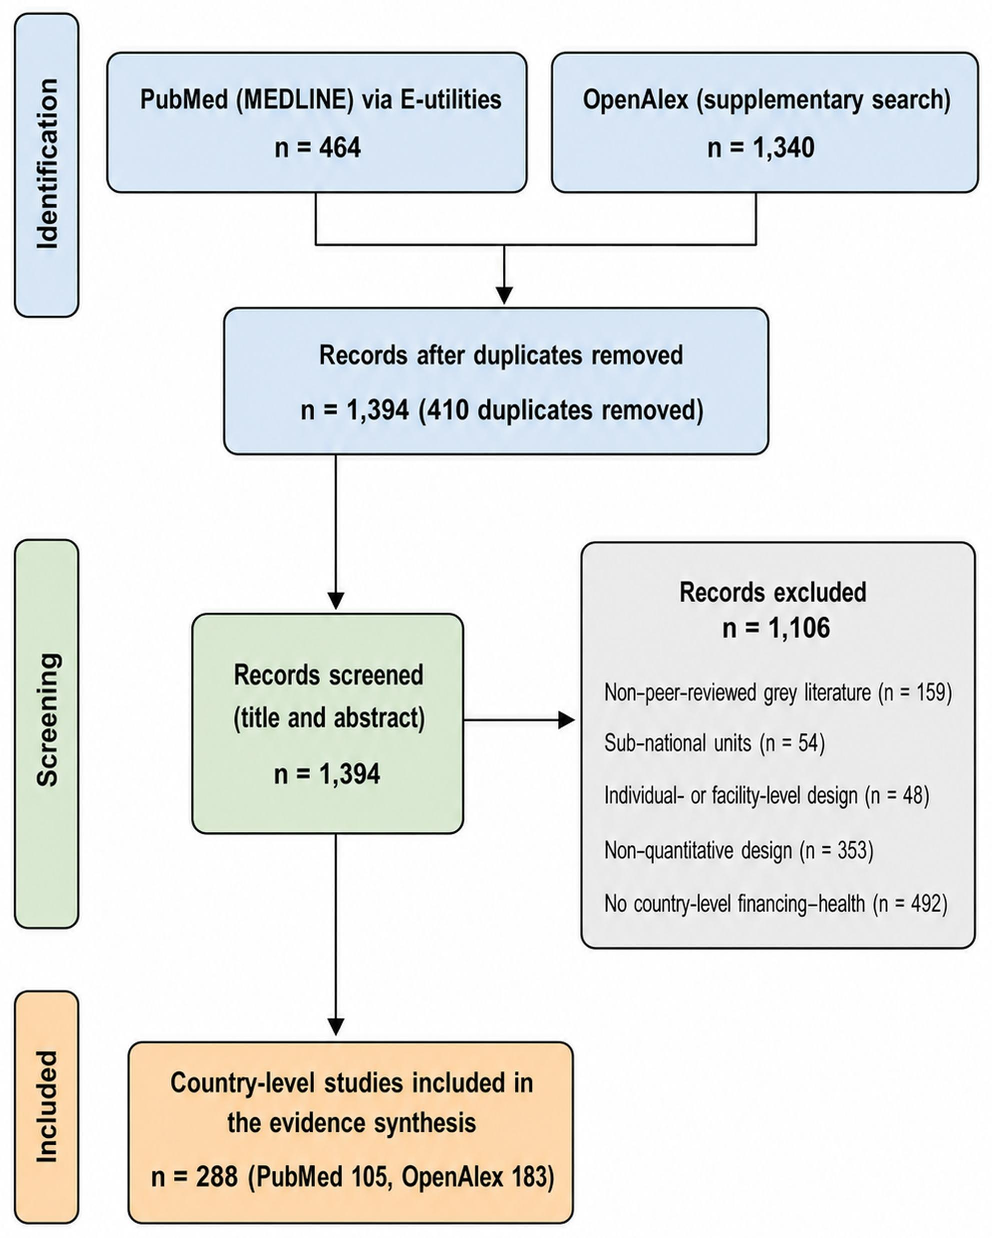
\includegraphics[width=0.85\textwidth]{../results/figures/figS1_prisma.pdf}
\caption{\textbf{PRISMA flow diagram.} Structured literature search and screening process. The search was conducted in PubMed (MEDLINE) through E-utilities on August 14, 2026, and identified 155 records (no duplicates). All 155 records were screened on title and abstract; 126 were excluded (no GHE exposure, $n = 16$; sub-national design only, $n = 31$; no health outcome, $n = 18$; review or commentary without original analysis, $n = 61$), and 29 studies were included in the evidence synthesis. The complete screening ledger is in the replication package.}
\label{fig:S1}
\end{figure}

\begin{figure}[H]\centering
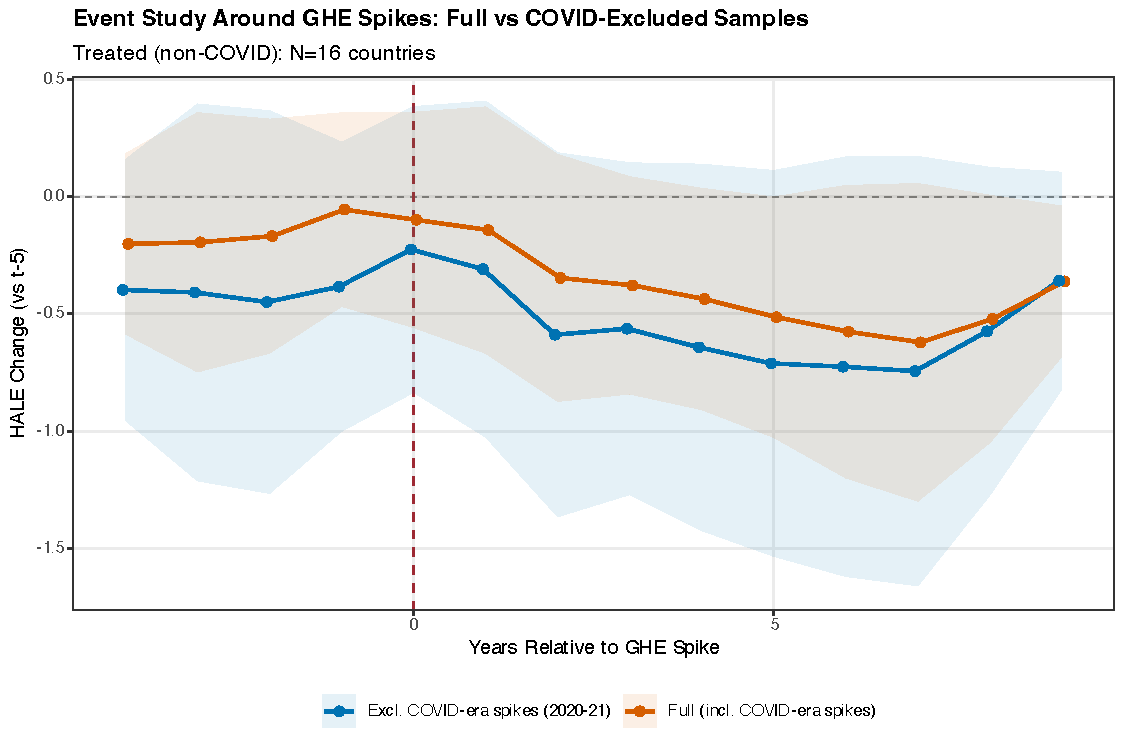
\includegraphics[width=0.85\textwidth]{../results/figures/figA1_event_study_nocovid.pdf}
\caption{\textbf{Event study excluding COVID-era GHE spikes (2020--2021).} HALE trajectory around non-COVID GHE spike episodes. Nine COVID-era spikes (Cyprus, UK, Libya, Montenegro, Russia, USA in 2020; Cabo Verde, Latvia, Mongolia in 2021) were excluded to isolate the structural relationship from pandemic-era spending surges. The remaining treated countries ($N = 16$) show a persistent negative post-spike HALE trajectory, compatible with crisis-related spending responses and not driven exclusively by pandemic-era hospital spending. Pre-trend $p > 0{\textperiodcentered{}}3$; SE clustered at country level.}
\label{fig:S2}
\end{figure}

\begin{figure}[H]\centering
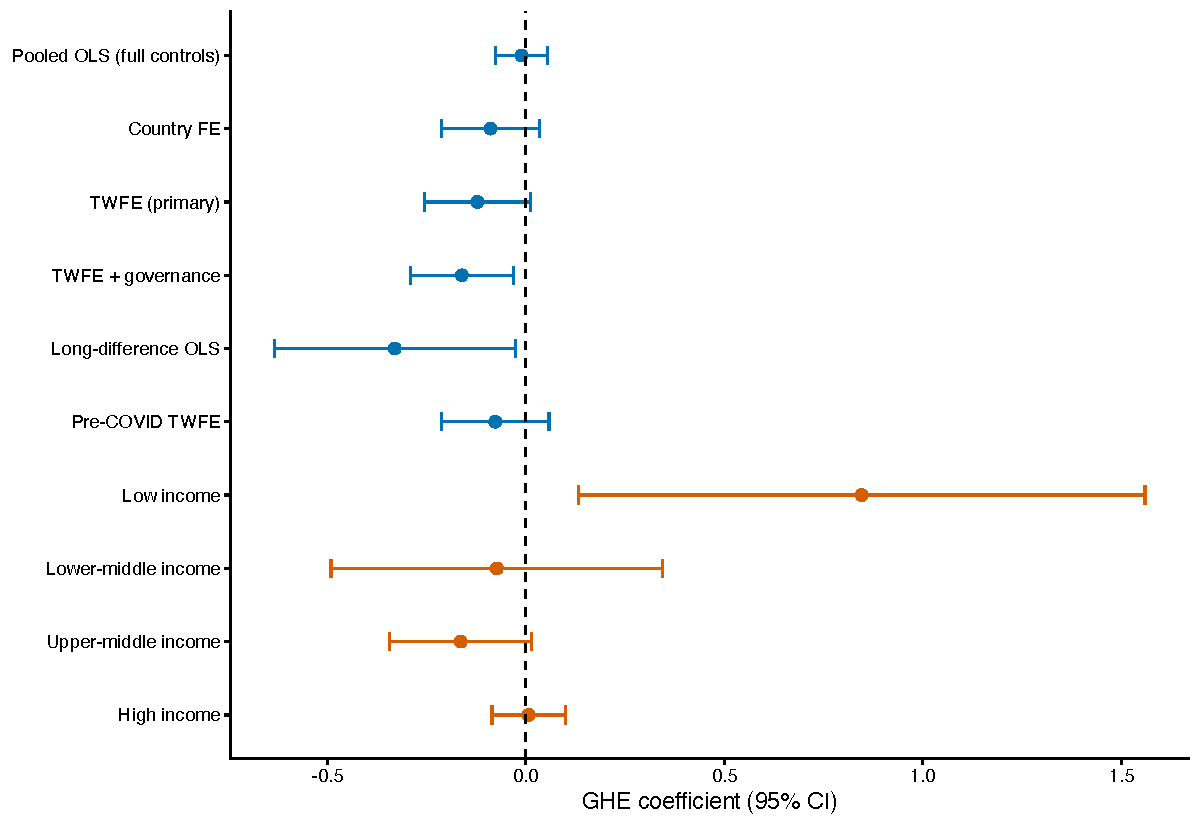
\includegraphics[width=0.9\textwidth]{../results/figures/fig2_forest.pdf}
\caption{\textbf{Coefficient forest plot.} GHE--HALE association across all TWFE specifications and income subgroups. Specifications include: (1) Pooled OLS with full controls, (2) Country FE only, (3) TWFE primary, (4) TWFE with governance controls, (5) Long-difference OLS, (6) Pre-COVID TWFE, (7--10) Income-group stratified TWFE. Error bars represent 95\% confidence intervals with standard errors clustered at the country level. All within-country estimates are negative or null except the low-income stratified estimate. The between-country OLS estimate is large and positive ($+1{\textperiodcentered{}}47$), illustrating the severity of cross-sectional confounding.}
\label{fig:S3}
\end{figure}

\begin{figure}[H]\centering
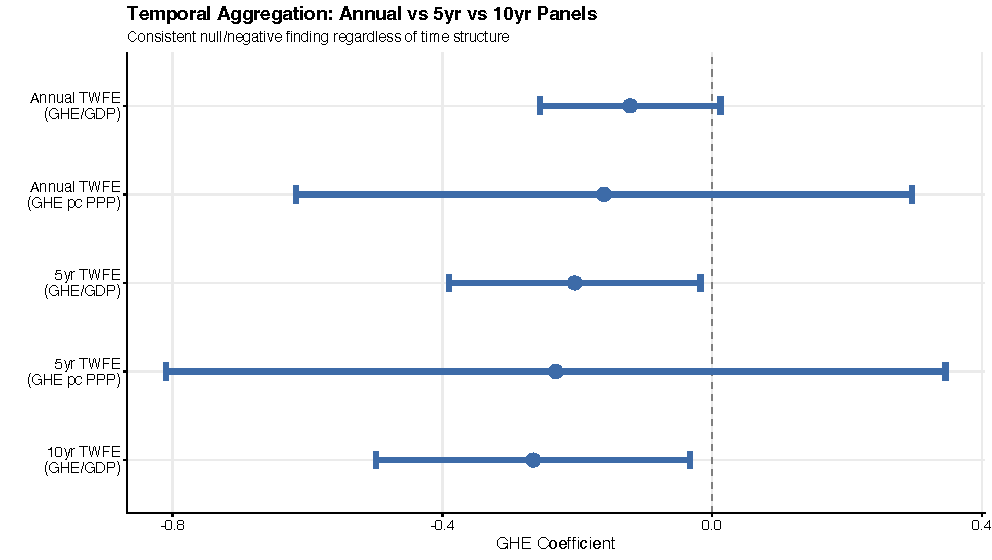
\includegraphics[width=0.9\textwidth]{../results/figures/fig8_temporal_aggregation.pdf}
\caption{\textbf{Temporal aggregation.} GHE--HALE TWFE coefficients across annual, 5-year averaged, and 10-year averaged panel specifications. All models include country and period fixed effects with full controls. The null finding is consistent across temporal resolutions: annual ($\beta = -0{\textperiodcentered{}}122$, $p = 0{\textperiodcentered{}}077$), 5-year ($\beta = -0{\textperiodcentered{}}204$, $p = 0{\textperiodcentered{}}034$), and 10-year ($\beta = -0{\textperiodcentered{}}265$, $p = 0{\textperiodcentered{}}027$). Temporal aggregation reduces measurement error and year-to-year noise. The strengthening of the negative coefficient with aggregation is inconsistent with the hypothesis that the null result is driven by measurement error.}
\label{fig:S4}
\end{figure}

\begin{figure}[H]\centering
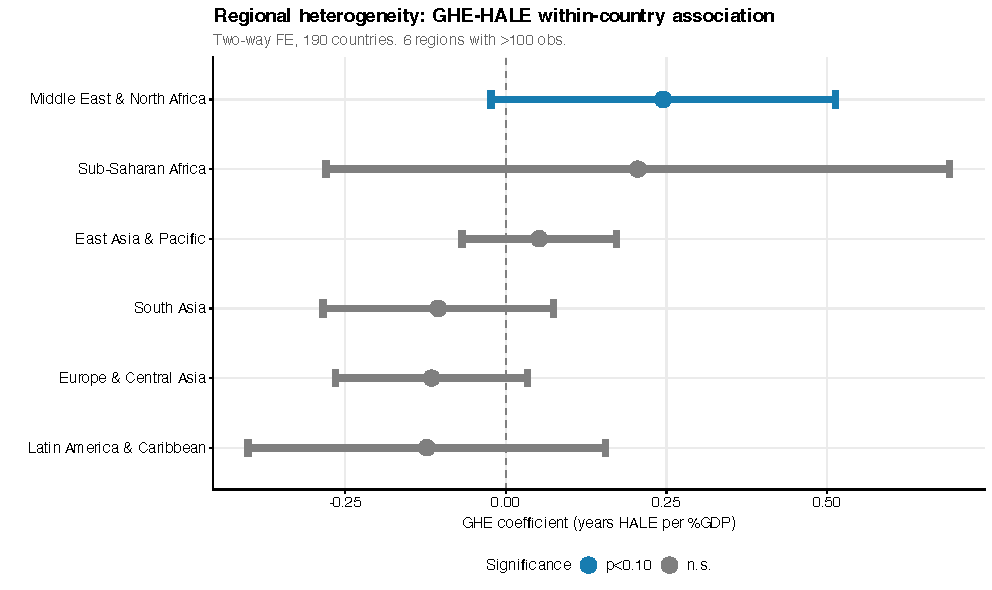
\includegraphics[width=0.9\textwidth]{../results/figures/fig7_regional.pdf}
\caption{\textbf{Regional heterogeneity.} TWFE GHE--HALE coefficients stratified by World Bank region. Sub-Saharan Africa and Middle East \& North Africa are the only regions with positive within-country coefficients. This pattern is consistent with the income-group findings: SSA contains 21 of 24 baseline-classified low-income countries in the sample (the remaining three are Afghanistan, Syria, and Yemen). The positive SSA coefficient ($+0{\textperiodcentered{}}21$, $p = 0{\textperiodcentered{}}411$) was positive but not statistically significant and likely reflects the same low-income mechanism identified in the stratified analysis. The negative coefficients in Europe \& Central Asia, East Asia \& Pacific, and Latin America \& Caribbean are consistent with the null overall finding.}
\label{fig:S5}
\end{figure}

\begin{figure}[H]\centering
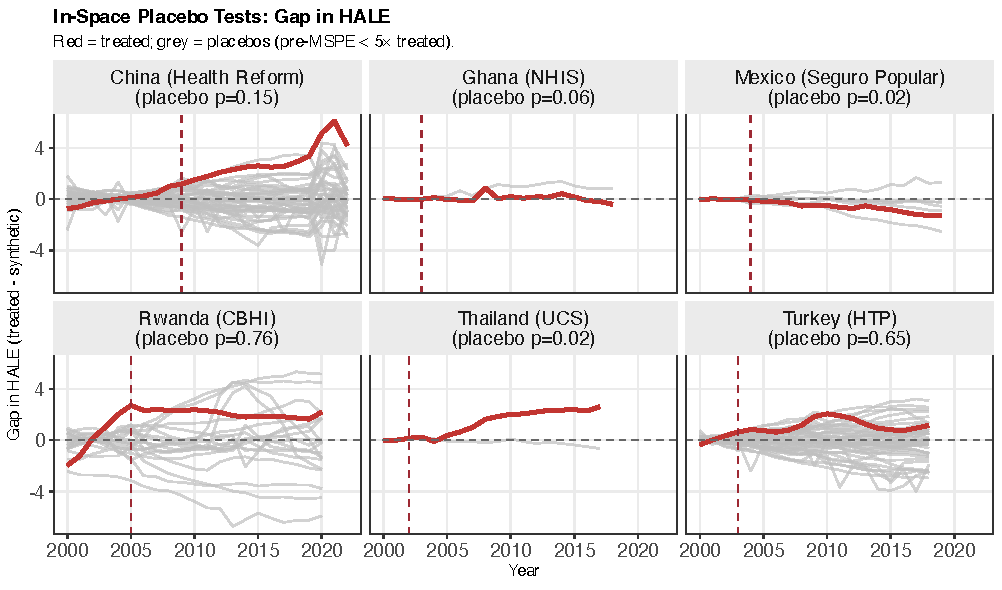
\includegraphics[width=0.9\textwidth]{../results/figures/A2_synth_gaps.pdf}
\caption{\textbf{Synthetic control gap plots.} Difference between observed HALE and synthetic counterfactual for six major health financing reforms. Red line: treated country. Grey lines: placebo donor-pool countries (iteratively assigned treatment). Dashed vertical line: reform year. Positive gaps indicate HALE improvements relative to the counterfactual. Only Rwanda (CBHI) and China (2009 reform) show sustained positive post-reform gaps, though pre-treatment fit limitations caution against strong causal interpretations for China and Thailand.}
\label{fig:S6}
\end{figure}

\begin{figure}[H]\centering
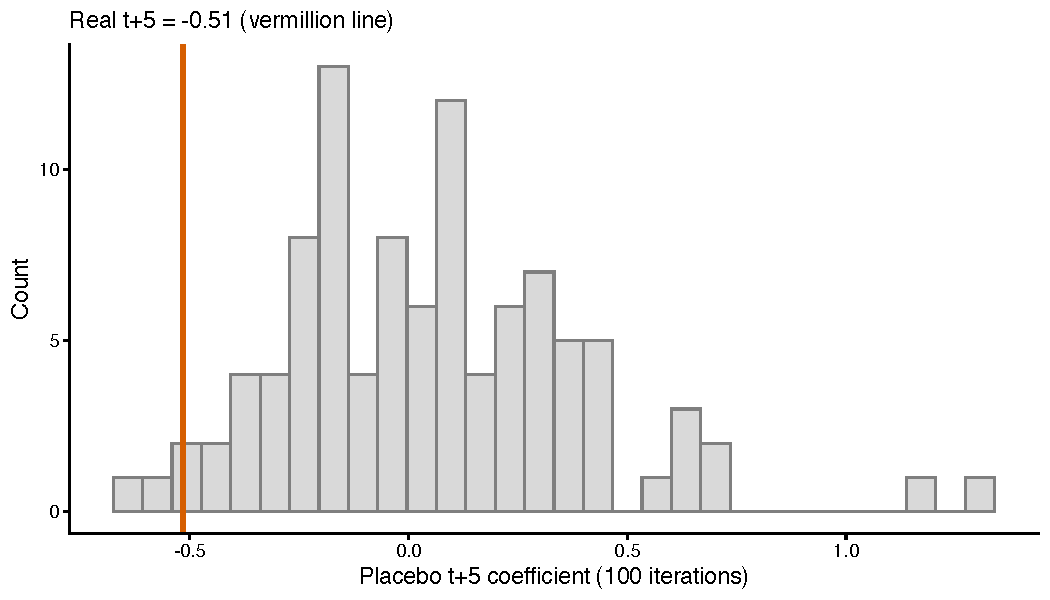
\includegraphics[width=0.9\textwidth]{../results/figures/B2_placebo_distribution.pdf}
\caption{\textbf{Placebo event study distribution.} Distribution of placebo event-study coefficients at $t+5$ from 100 iterations with randomly assigned pseudo-event years. Each iteration randomly assigns pseudo-spike years (drawn from the observed event-year distribution) to an equal number of untreated countries and re-estimates the full event study. Only 1\% of placebo iterations produced significant negative effects. The real event-study coefficient lies at the 3rd percentile of the placebo distribution, indicating the observed pattern is unlikely to arise by chance.}
\label{fig:S7}
\end{figure}

\begin{figure}[H]\centering
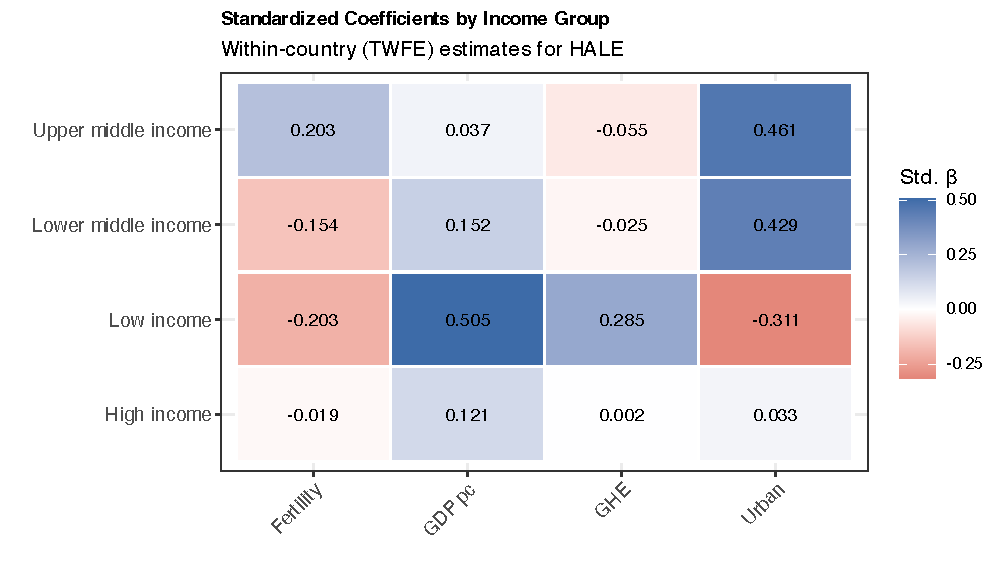
\includegraphics[width=0.9\textwidth]{../results/figures/C4_horse_race_income.pdf}
\caption{\textbf{Standardised coefficients by income group.} Within-country (TWFE) standardised predictors of HALE stratified by World Bank income classification. All variables $z$-standardised within each income group before estimation. Colour scale represents standardised coefficient magnitude: orange (positive), white (null), blue (negative). Fertility is the dominant predictor across all income groups. GHE coefficients range from $+0{\textperiodcentered{}}286$ (low-income, $p = 0{\textperiodcentered{}}030$) to $+0{\textperiodcentered{}}002$ (high-income, $p = 0{\textperiodcentered{}}882$). The low-income GHE coefficient is the second-strongest predictor in that group (after GDP per capita), consistent with the income-stratified TWFE results.}
\label{fig:S8}
\end{figure}

\begin{figure}[H]\centering
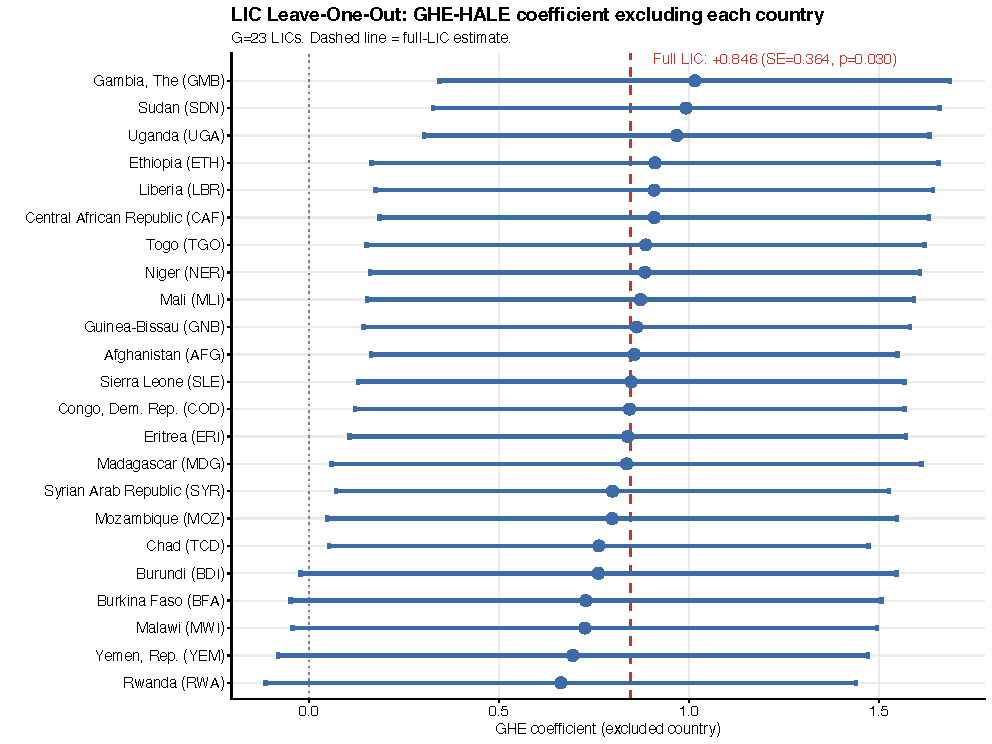
\includegraphics[width=0.9\textwidth]{../results/figures/LGH1_lic_loo.pdf}
\caption{\textbf{LIC leave-one-out analysis.} GHE--HALE TWFE coefficient excluding each low-income country in turn. The y-axis lists the excluded country, ordered by the re-estimated coefficient; the x-axis shows the coefficient with its 95\% confidence interval. All 23 leave-one-out point estimates remain positive; corresponding 95\% confidence intervals span zero for most countries (range $+0{\textperiodcentered{}}663$ to $+1{\textperiodcentered{}}016$), confirming no single LIC drives the overall result. The dashed vertical line marks the full-LIC TWFE estimate ($\beta = +0{\textperiodcentered{}}846$; clustered $p = 0{\textperiodcentered{}}030$). The narrow spread of estimates demonstrates that the positive LIC signal is broadly distributed across countries rather than concentrated in a few influential outliers.}
\label{fig:S9}
\end{figure}

\begin{figure}[H]\centering
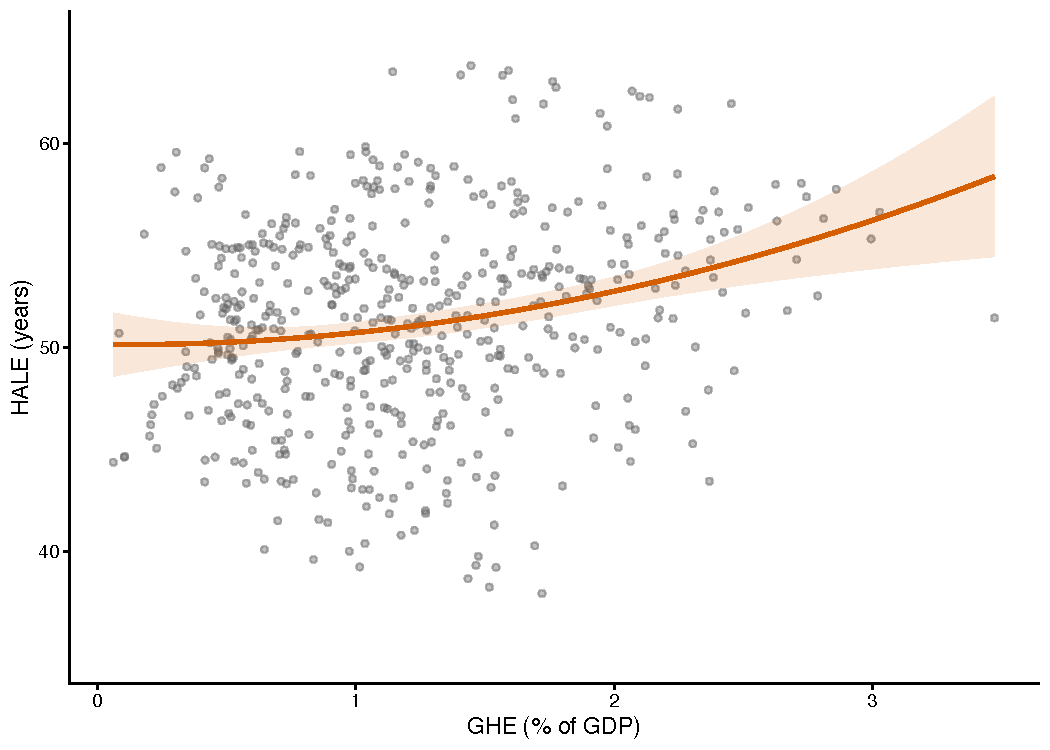
\includegraphics[width=0.9\textwidth]{../results/figures/LGH2_lic_doseresponse.pdf}
\caption{\textbf{LIC dose-response.} Quadratic fit of GHE (\% of GDP) versus HALE in low-income countries, with 95\% confidence band (grey shading). Each point represents one country-year observation. The positive quadratic term ($+0{\textperiodcentered{}}52$, $p = 0{\textperiodcentered{}}027$) indicates a convex dose-response, with the marginal HALE association larger at higher GHE levels; this shape is driven by a small number of high-GHE observations and should be interpreted cautiously, and the pattern is attenuated when Rwanda is excluded.}
\label{fig:S10}
\end{figure}

\begin{figure}[H]\centering
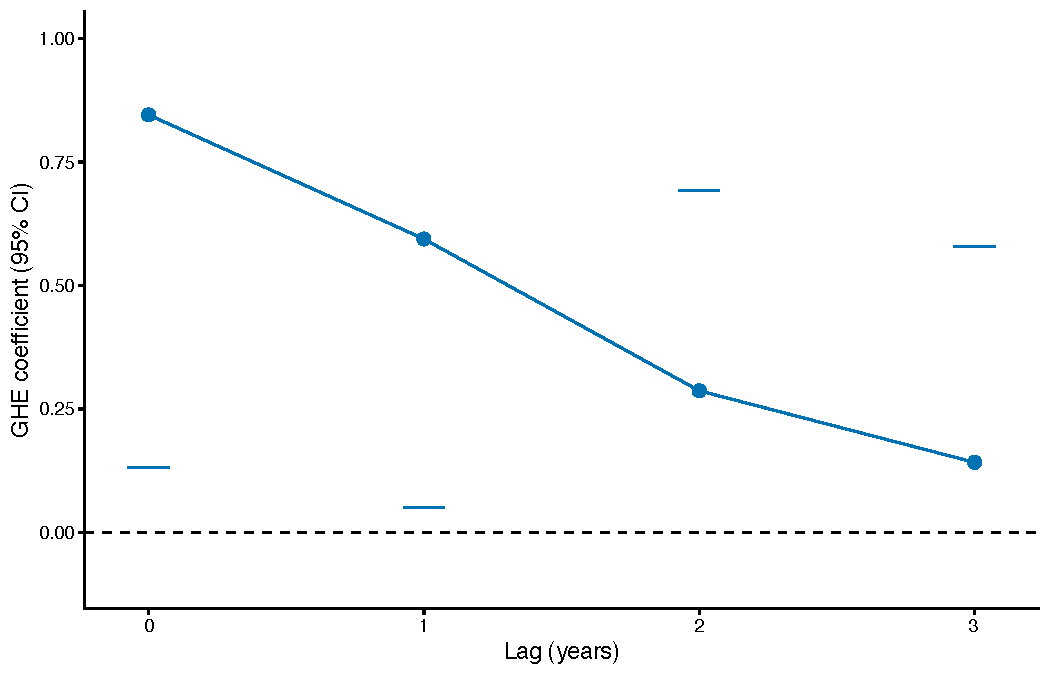
\includegraphics[width=0.9\textwidth]{../results/figures/LGH3_lic_lagstructure.pdf}
\caption{\textbf{LIC lag structure.} GHE measured at contemporaneous ($t$) and lagged 1--3 years in the low-income TWFE specification. All models include country and year fixed effects with full controls. The association peaks at contemporaneous GHE ($\beta = +0{\textperiodcentered{}}846$, $p = 0{\textperiodcentered{}}030$) and decays monotonically: 1-year lag ($\beta = +0{\textperiodcentered{}}594$, $p = 0{\textperiodcentered{}}044$), 2-year lag ($\beta = +0{\textperiodcentered{}}287$, $p = 0{\textperiodcentered{}}180$), 3-year lag ($\beta = +0{\textperiodcentered{}}142$, $p = 0{\textperiodcentered{}}532$). This contemporaneous-peak pattern is consistent with, but does not prove, a forward-causal mechanism: coincident measurement and common time trends could also produce this pattern. If poor health outcomes drove subsequent spending increases, we would expect lagged coefficients to be larger than the contemporaneous one.}
\label{fig:S11}
\end{figure}

\begin{figure}[H]\centering
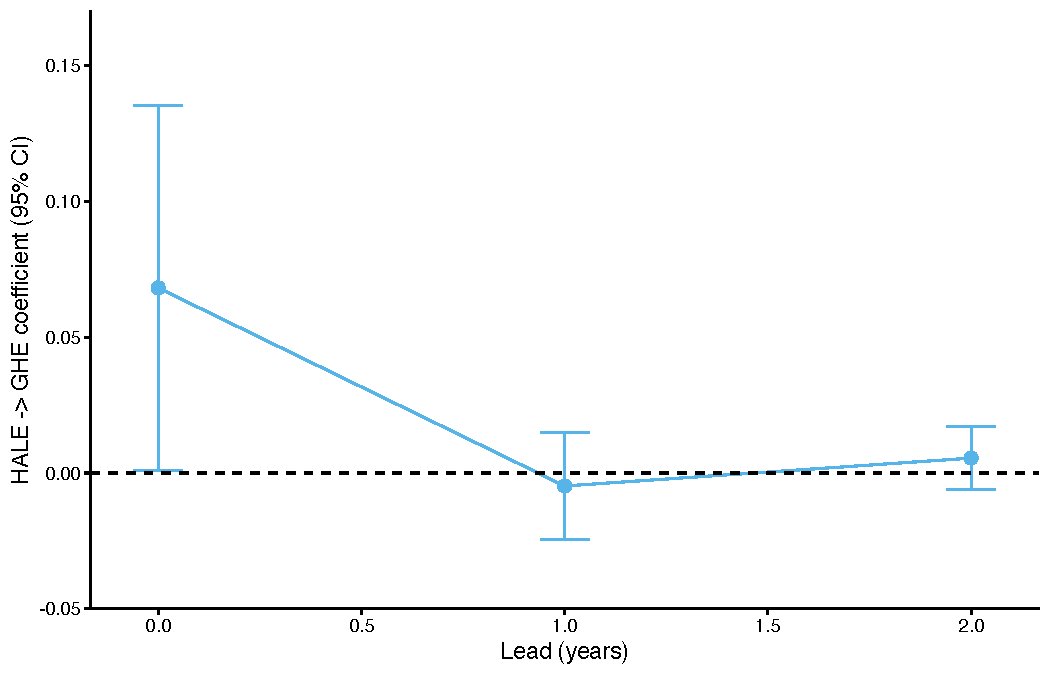
\includegraphics[width=0.9\textwidth]{../results/figures/LGH4_lic_reversecausality.pdf}
\caption{\textbf{LIC reverse causality check.} Past HALE as a predictor of current GHE in low-income countries. Contemporaneous HALE: $\beta = +0{\textperiodcentered{}}068$, $p = 0{\textperiodcentered{}}059$ (borderline). HALE lag-1 (HALE at $t-1$ predicting GHE at $t$): $\beta = -0{\textperiodcentered{}}005$, $p = 0{\textperiodcentered{}}643$. HALE lag-2 (HALE at $t-2$): $\beta = +0{\textperiodcentered{}}006$, $p = 0{\textperiodcentered{}}360$. The non-significance of lagged HALE in predicting future GHE provides no evidence that poor health outcomes drive subsequent increases in government health spending. The borderline contemporaneous association is expected; it reflects the same GHE--HALE relationship identified in the primary TWFE specification, not a distinct reverse-causality pathway. All models include country and year fixed effects with full controls.}
\label{fig:S12}
\end{figure}

\begin{figure}[H]\centering
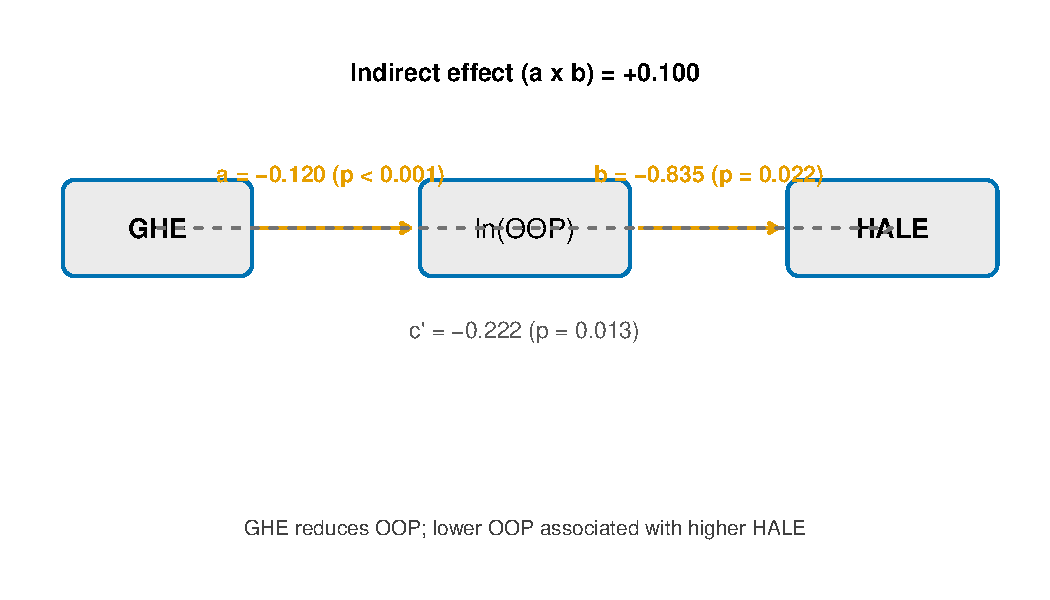
\includegraphics[width=0.9\textwidth]{../results/figures/S13_oop_pathway.pdf}
\caption{\textbf{OOP mediation pathway.} Mediation analysis of GHE $\rightarrow$ OOP $\rightarrow$ HALE under two-way fixed effects. Path a (GHE $\rightarrow$ ln OOP): $\beta = -0{\textperiodcentered{}}120$ ($p < 0{\textperiodcentered{}}001$), a semi-elasticity indicating that each percentage point of GDP in GHE is associated with an approximate 11\% relative reduction in the OOP share. Path b (ln OOP $\rightarrow$ HALE): $\beta = -0{\textperiodcentered{}}835$ ($p = 0{\textperiodcentered{}}022$), indicating that lower OOP is associated with higher HALE. Direct path $c' = -0{\textperiodcentered{}}222$ ($p = 0{\textperiodcentered{}}013$); indirect effect $a \times b = +0{\textperiodcentered{}}100$. The indirect effect ($a \times b = +0{\textperiodcentered{}}100$) partially offsets the negative direct effect ($c' = -0{\textperiodcentered{}}222$), so the total effect is $c = -0{\textperiodcentered{}}122$. This pattern indicates that GHE is associated with a lower OOP share even where it is not associated with measurable HALE gains.}
\label{fig:S13}
\end{figure}

\begin{figure}[H]\centering
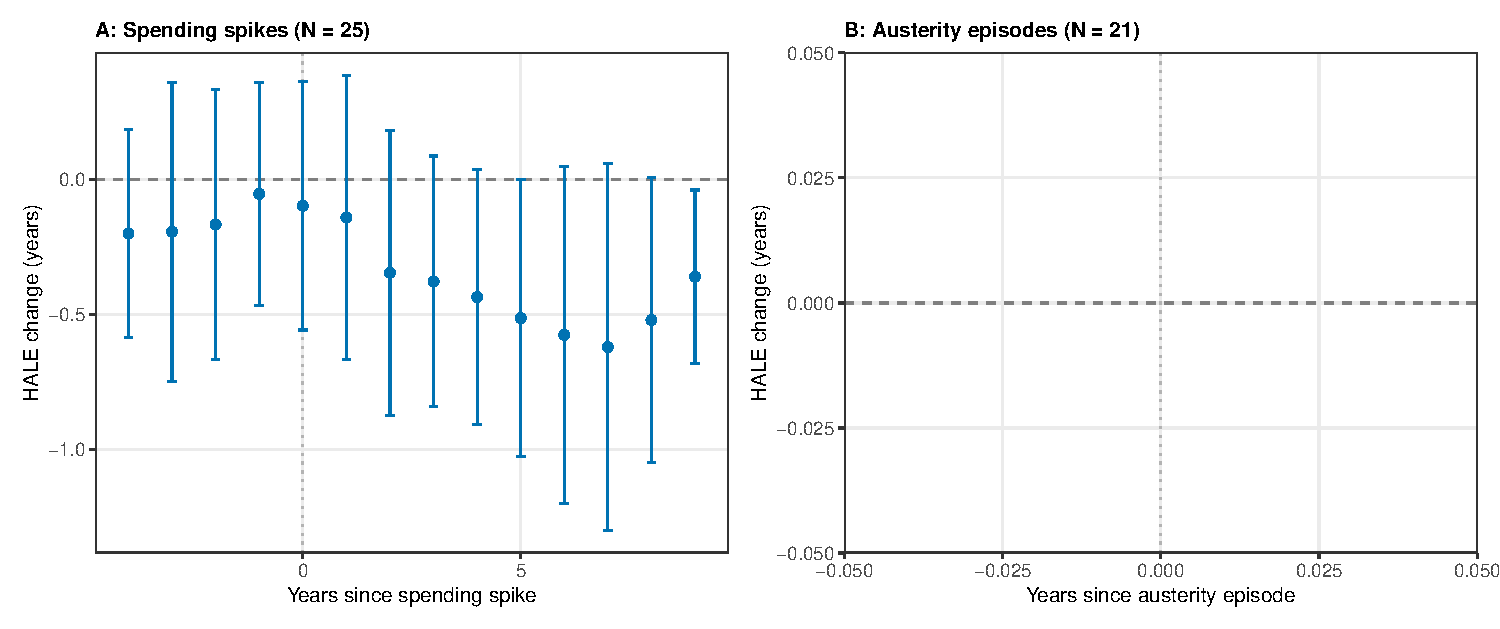
\includegraphics[width=0.9\textwidth]{../results/figures/fig2_event_austerity.pdf}
\caption{\textbf{Event study: HALE trajectory around GHE spikes and austerity episodes.}
\textbf{A:} GHE spikes ($>2$ percentage points of GDP within three years; $N = 25$ treated countries). HALE declined progressively after the spike, reaching $-0{\textperiodcentered{}}49$ years at $t+5$ ($p = 0{\textperiodcentered{}}037$), a pattern compatible with crisis-related spending responses; excluding COVID-era spikes ($N = 16$) the $t+5$ estimate was $-0{\textperiodcentered{}}54$ ($p = 0{\textperiodcentered{}}094$). \textbf{B:} Austerity episodes ($>1{\textperiodcentered{}}5$ percentage point cuts within three years; $N = 21$ treated countries). Post-austerity HALE showed no significant change ($t+5$: $+0{\textperiodcentered{}}17$, $p = 0{\textperiodcentered{}}39$; post-average $+0{\textperiodcentered{}}17$); the asymmetry, with declines after surges but not after cuts, is compatible with crisis-driven covariation between fiscal responses and health shocks rather than direct effects of spending changes. Error bars are 95\% confidence intervals with standard errors clustered at the country level.}
\label{fig:S14}
\end{figure}



\section*{Funding}
National Natural Science Foundation of China (82403759 to CX; 82403616 to YW). CX and YW provided the research funding through these grants and participated in the data analysis.

\section*{Supplementary References}
\begin{enumerate}[leftmargin=*, label=S\arabic*.]
\item[S1.] Cameron AC, Gelbach JB, Miller DL. Bootstrap-based improvements for inference with clustered errors. \textit{Rev Econ Stat} 2008; \textbf{90}: 414--27.
\item[S2.] Lakens D. Equivalence tests: a practical primer. \textit{Soc Psychol Personal Sci} 2017; \textbf{8}: 355--62.
\item[S3.] van Buuren S, Groothuis-Oudshoorn K. mice: MICE in R. \textit{J Stat Softw} 2011; \textbf{45}: 1--67.
\item[S4.] Abadie A, Diamond A, Hainmueller J. Synthetic control methods for comparative case studies. [Cited as reference 23 in the main text.]
\item[S5.] Boundioa J, et al. Threshold effect of governance quality in the relationship between public health expenditure and life expectancy. \textit{BMC Health Serv Res} 2025; \textbf{25}: 432. PMID 40140811.
\item[S6.] Kabongo WNS, Mbonigaba J. Effectiveness of public health spending. [Cited as reference 30 in the main text.] PMID 38978095.
\item[S7.] Zeng M, et al. Spatiotemporal patterns of healthy life expectancy and the effects of health financing in West African countries. \textit{J Glob Health} 2023; \textbf{13}: 04123. PMID 37861131.
\item[S8.] Boundioa J, et al. Effect of public health expenditure on maternal mortality ratio in the West African Economic and Monetary Union. \textit{BMC Womens Health} 2024; \textbf{24}: 109. PMID 38336729.
\item[S9.] Jan A, et al. Impact of government health expenditure on maternal mortality: an appraisal of South Asian economies. \textit{Inquiry} 2025; \textbf{62}: 469580251339069. PMID 40717485.
\item[S10.] Liang LL, Mirelman AJ. The cyclicality of government health expenditure and its effects on population health. \textit{Health Policy} 2019; \textbf{123}: 96--103. PMID 30482387.
\item[S11.] Fujii T. Sources of health financing and health outcomes: a panel data analysis. \textit{Health Econ} 2018; \textbf{27}: 1996--2015. PMID 30112851.
\item[S12.] Raeesi P, et al. Effects of private and public health expenditure on health outcomes among countries with different health care systems: 2000--2014. \textit{Med J Islam Repub Iran} 2018; \textbf{32}: 35. PMID 30159286.
\item[S13.] Moreno-Serra R, Smith PC. Broader health coverage is good for the nation's health: evidence from country level panel data. \textit{J R Stat Soc Ser A Stat Soc} 2015; \textbf{178}: 101--24. PMID 25598588.
\item[S14.] Makuta I, O'Hare B. Quality of governance, public spending and health. [Cited as reference 15 in the main text.]
\item[S15.] MacKinnon DP, Lockwood CM, Hoffman JM, West SG, Sheets V. A comparison of methods to test mediation and other intervening variable effects. \textit{Psychol Methods} 2002; \textbf{7}: 83--107.
\item[S16.] von Elm E, Altman DG, Egger M, Pocock SJ, Gøtzsche PC, Vandenbroucke JP. The Strengthening the Reporting of Observational Studies in Epidemiology (STROBE) statement: guidelines for reporting observational studies. \textit{PLoS Med} 2007; \textbf{4}: e296.
\item[S17.] Stevens GA, Alkema L, Black RE, et al. Guidelines for Accurate and Transparent Health Estimates Reporting: the GATHER statement. \textit{Lancet} 2016; \textbf{388}: e19--e23.
\end{enumerate}

\end{document}
